\documentclass[10pt,twocolumn]{article}

\usepackage[margin=0.72in,columnsep=0.25in]{geometry}
\usepackage[T1]{fontenc}
\usepackage{lmodern}
\usepackage{microtype}
\usepackage{graphicx}
\usepackage{booktabs}
\usepackage{tabularx}
\usepackage{array}
\usepackage{indentfirst}
\usepackage{amsmath,amssymb}
\usepackage{enumitem}
\usepackage{url}
\usepackage{hyperref}
\usepackage[round,authoryear]{natbib}
\usepackage{caption}
\usepackage{tikz}
\usetikzlibrary{arrows.meta,positioning,fit}

\hypersetup{colorlinks=true,linkcolor=black,citecolor=black,urlcolor=black}
\captionsetup{font=small,labelfont=bf}
\setlength{\parindent}{1.25em}
\setlength{\parskip}{0pt}
\setlist[itemize]{leftmargin=1.2em,itemsep=1pt,topsep=2pt}
\setcounter{tocdepth}{2}
\setcounter{secnumdepth}{2}
\renewcommand{\contentsname}{Contents}

\title{\textbf{Structured Episodic Memory (SEM)}}
\author{Berat D. Ara\c{c}\\Independent Researcher}
\date{September 2026}

\begin{document}
\onecolumn
\hypersetup{pageanchor=false}
\pagenumbering{gobble}

% -----------------------------------------------------------------------------
% Front matter
% -----------------------------------------------------------------------------
\begin{titlepage}
\thispagestyle{empty}
\centering
\vspace*{0.14\textheight}
{\Large\scshape Research Paper\par}
\vspace{1.5cm}
{\Huge\bfseries Structured Episodic Memory (SEM)\par}
\vspace{1.2cm}
\rule{0.68\textwidth}{0.6pt}\par
\vspace{1.4cm}
{\Large Berat D. Ara\c{c}\par}
\vspace{0.25cm}
{\large Independent Researcher\par}
\vfill
{\large September 2026\par}
\vspace{0.25cm}
{\normalsize Version 1.0\par}
\end{titlepage}

\clearpage
\hypersetup{pageanchor=true}
\pagenumbering{roman}
\setcounter{page}{1}
\tableofcontents
\clearpage

\section*{Abbreviations and Notation}
\addcontentsline{toc}{section}{Abbreviations and Notation}
\noindent This page collects the abbreviations, mathematical symbols, and experiment-phase labels used throughout the paper.

\vspace{0.8em}
\subsection*{Abbreviations}
\begin{tabularx}{\textwidth}{@{}>{\bfseries}p{0.16\textwidth}X@{}}
SEM & Structured Episodic Memory \\
RL & Reinforcement Learning \\
CMAC & Cerebellar Model Articulation Controller \\
MAE & Mean Absolute Error \\
DQN & Deep Q-Network \\
JSON & JavaScript Object Notation \\
\end{tabularx}

\vspace{1em}
\subsection*{Core notation}
\begin{tabularx}{\textwidth}{@{}p{0.22\textwidth}X@{}}
$\mathcal{A}_m$ & Discrete survival-motor action set controlling paddle velocity. \\
$\mathcal{A}_c$ & Discrete contact-intention set used to bias where the paddle contacts the ball. \\
$v_x, v_y$ & Current horizontal and vertical ball velocity. \\
$F, S$ & Fast and slow exponential action-value estimates stored in associative memory. \\
$Q_{\mathrm{survival}}$ & Aggregated survival-motor value used to reach the incoming ball. \\
$Q_{\mathrm{aim}}$ & Goal-conditioned residual value used to alter contact location. \\
$c$ & Actual normalized paddle-ball contact location. \\
$g$ & Requested normalized contact intention. \\
\end{tabularx}

\vspace{1em}
\subsection*{Experiment-phase labels}
\begin{tabularx}{\textwidth}{@{}p{0.22\textwidth}X@{}}
A1 / B / A2 & Initial condition, hidden changed condition, and return to the initial condition. The agent receives no phase identifier. \\
B1 / B2 & First and repeated exposure to the hidden inverted actuator mapping in retention experiments. \\
Frozen checkpoint & Evaluation in which learned values are loaded but no further value updates are permitted. \\
Incoming outcome & One ball approach toward SEM ending in either a paddle hit or a miss. \\
\end{tabularx}

\clearpage
\pagenumbering{arabic}
\setcounter{page}{1}
\addcontentsline{toc}{section}{Abstract}
\twocolumn[
\begin{@twocolumnfalse}
\begin{abstract}
This paper presents Structured Episodic Memory (SEM), an experimental agent architecture that learns Pong control and opponent responsive behavior without a neural policy and without an analytical future trajectory solver. SEM receives engineered current frame state variables, converts them into multiple overlapping discrete abstractions, and stores action values in associative tables. A survival motor memory learns to reach the ball from sparse hit or miss outcomes, a goal conditioned residual memory learns to alter contact location, and an opponent response memory selects contact intentions online. Credit for delayed motor outcomes is assigned through bounded, decaying eligibility traces over motor decisions. Fast and slow value estimates provide multiple update timescales, although experiments show that the present slow component has only modest support.

Across a 40-run curriculum containing 2,200 incoming ball outcomes, the first run achieved a 0.709 hit rate and a frozen evaluation on six fresh seeds reached a mean hit rate of 0.974. Controlled ablations show that temporal eligibility traces improve late motor performance, the aiming memory substantially improves goal-conditioned contact control, fast value estimates accelerate adaptation after hidden opponent changes, and context-specific strategy memory is required for high performance in a conflicting-context benchmark where the same action has opposite value in different observable contexts. Under a simultaneous physics shift, a frozen checkpoint retains a 0.921 hit rate. An abstraction ablation yields 0.945 hit rate with the full overlapping representation and 0.929 with coarse abstractions alone, compared with 0.564 when only the most specific key is available. When the actuator mapping is secretly inverted, performance falls to 0.175 in the first 20 outcomes and recovers to 0.733 in the last 20. Repeated exposure reduces mean reacquisition latency from 158.8 to 91.7 outcomes; in addition, the repeated-exposure condition has higher first-50 and first-100 hit rates than a matched-experience control encountering the inversion for the first time.

SEM is not presented as blank slate pixel learning, a biologically realistic memory model, or a replacement for standard reinforcement learning. Its contribution is a controlled study of how structured associative memory, overlapping abstractions, and sparse temporal credit can compose into adaptive behavior without neural function approximation.
\end{abstract}
\vspace{0.8em}
\end{@twocolumnfalse}
]

\section{Introduction}
Deep reinforcement learning has demonstrated that a learned neural representation and a value or policy learner can jointly solve control problems directly from high dimensional observations \citep{mnih2015dqn}. This success can obscure a simpler question: how much adaptive behavior can be obtained when the policy itself is not a neural network, and when useful structure is placed in memory organization, temporal credit assignment, and overlapping state abstraction instead?

Structured Episodic Memory, abbreviated SEM, was built as an experimental answer to that question. The system is intentionally small and inspectable. It observes current Pong state variables such as ball position, ball velocity, paddle position, and speed. It does not estimate a future paddle intersection, does not simulate future wall bounces, and does not receive a target interception coordinate. Instead, current observations address several overlapping associative keys. Action values stored under those keys are updated only after sparse physical outcomes. The term \emph{episodic} refers to these outcome bounded interaction segments and their temporary eligibility traces. It does not imply human autobiographical memory or a claim of biological equivalence.

None of the individual ingredients is new in isolation. Tabular value learning, temporal difference methods, eligibility traces, coarse coding, and episodic control all have long histories \citep{sutton1988td,watkins1992q,sutton2018rl,sutton1996coarse,albus1975cmac,blundell2016mfec,pritzel2017nec}. The purpose of this work is therefore not to claim a new learning principle. The contribution is the composition of these ideas into a compact control architecture, followed by controlled ablation and distribution-shift tests that attempt to separate what each part actually contributes.

The experimental program asks five questions. First, can sparse hit or miss outcomes produce useful motor behavior without an analytical trajectory oracle? Second, does temporal credit over preceding actions matter? Third, can a separate goal conditioned memory change where the paddle contacts the ball while preserving interception? Fourth, can outcome memories adapt when opponent response statistics or actuator consequences change without warning? Fifth, does the overlapping representation transfer beyond exact state lookup under shifted physics?

The resulting evidence supports affirmative answers to all five questions in the tested Pong setting, with important boundaries. SEM is given engineered state variables and bins. The action vocabulary, incoming ball gate, reward definitions, and actuator smoothing are also engineered. The system is therefore not a blank slate learner. In addition, the current slow value estimate has only weak stabilization evidence and should not be treated as a central validated advantage.

\section{Related Work}
\subsection{Tabular control and temporal credit}
Classical reinforcement learning studies incremental value estimation and control under delayed reward \citep{sutton1988td,watkins1992q,sutton2018rl}. Eligibility traces provide one established mechanism for assigning later outcomes to earlier state action decisions. SEM uses a related but simpler mechanism: it maintains a bounded replacing trace over recent motor decisions, decays it between decisions, and applies the eventual sparse hit or miss target to all surviving trace entries. It does not bootstrap from a next state value and is not presented as an implementation of Q learning or Sarsa $\lambda$.

\subsection{Coarse coding and associative control}
SEM's overlapping state keys are closely related in spirit to sparse coarse coding and CMAC style memory addressing. CMAC demonstrated that continuous control functions can be approximated by combining multiple overlapping table addresses \citep{albus1975cmac}. Sparse coarse coding was later studied explicitly as a generalization mechanism in reinforcement learning \citep{sutton1996coarse}. SEM uses several hand designed levels of discretization rather than a single exact state key. The experiments in Section~\ref{sec:generalization} directly test whether this overlap contributes to transfer.

\subsection{Episodic and memory based reinforcement learning}
Model Free Episodic Control and Neural Episodic Control showed that rapidly written value memories can complement slower parametric learning \citep{blundell2016mfec,pritzel2017nec}. SEM differs in two important ways. First, the representation used to address memory is engineered and discrete rather than a learned neural embedding. Second, the motor controller itself is an associative memory over overlapping abstractions, not a neural network supported by an episodic side memory.

\subsection{Memory-based and non-parametric reinforcement learning}
Explicit memory and local, non-parametric estimation have also appeared in reinforcement learning outside modern neural episodic-control systems. Moore and Atkeson used retained transition experience in prioritized sweeping to focus model-based dynamic-programming updates \citep{moore1992memory,moore1993prioritized}. Unemi proposed an instance-based reinforcement-learning method that stores past input-action experience and propagates delayed reinforcement backward through remembered interaction sequences \citep{unemi1992instance}. Ormoneit and Sen studied kernel-based reinforcement learning, using local averaging rather than a parametric value function in continuous state spaces \citep{ormoneit2002kernel}. These systems are relevant precedents for explicit-memory control, but they differ algorithmically from SEM: SEM does not learn a transition model for planning, does not retrieve raw nearest-neighbor episodes as its motor policy, and does not form kernel-smoothed Bellman backups. Its motor layer instead stores outcome-associated action values under several hand-designed overlapping keys and writes sparse outcomes backward through bounded eligibility traces.

\subsection{Continual adaptation}
Sequential learning can overwrite earlier competence, a problem commonly discussed as catastrophic interference or catastrophic forgetting \citep{mccloskey1989catastrophic,kirkpatrick2017ewc}. SEM does not include a dedicated continual learning regularizer. Instead, the retention tests in Section~\ref{sec:continual} ask whether partially distributed associative values leave measurable reacquisition savings after a previously learned actuator mapping disappears and later returns.

\section{Architecture}
\subsection{Observation and action interface}
The default environment is a deterministic 60 Hz Pong simulator with stochastic serves. The field is $1100\times650$ pixels, each paddle is $110$ pixels high, the base ball speed is 330 pixels per second, each paddle contact multiplies speed by 1.055 up to 1100 pixels per second, and the bounce angle is determined by actual contact position.

SEM controls the right paddle. It receives current frame values including ball position $(x_b,y_b)$, ball velocity $(v_x,v_y)$, ball speed, right paddle position, left paddle position, field dimensions, and paddle height. The survival motor action set is
\begin{equation}
\mathcal{A}_m=\{-1,-0.62,-0.28,0,0.28,0.62,1\},
\end{equation}
which is multiplied by the current maximum paddle speed. Contact intentions use
\begin{equation}
\mathcal{A}_c=\{-0.66,-0.44,-0.22,0,0.22,0.44,0.66\}.
\end{equation}
Positive and negative values correspond to normalized contact locations on the paddle.

The agent acts only while the ball is moving toward its side, identified by the engineered gate $v_x>0$. This gate is an explicit inductive bias and is not learned.

\subsection{Overlapping state abstractions}
For each motor decision, SEM computes binned features from current geometry. These include two distance resolutions, two relative vertical error resolutions, fine and signed vertical velocity, paddle and ball height bins, and a speed bin. Five keys are then generated from different subsets and resolutions of those features. The first key is the most specific and the final key is the coarsest. A single motor decision therefore addresses multiple associative entries.

For an action $a$ under key $k$, SEM stores count $n$, running mean, fast value $F$, and slow value $S$. After a target $z$ is observed,
\begin{align}
F &\leftarrow 0.66F+0.34z,\\
S &\leftarrow 0.945S+0.055z.
\end{align}
On the first update both values are initialized to $z$.

For a set of active keys $K(s)$, the base action estimate is a confidence weighted average,
\begin{equation}
\hat{Q}(s,a)=\frac{\sum_{k\in K(s)} w_k[0.70F_{k,a}+0.30S_{k,a}]}{\sum_{k\in K(s)}w_k},
\end{equation}
where $w_k$ decreases mildly with abstraction level and increases with evidence count. The survival table adds a symmetric uncertainty bonus proportional to $\sqrt{\log N/(1+n)}$, encouraging under sampled actions without privileging a movement direction.

\subsection{Sparse temporal credit}
Motor decisions are held for five rendered frames. Each new decision decays a replacing eligibility trace and inserts the currently active key action pairs with eligibility 1. The survival trace uses decay 0.88 and a maximum of 84 items. No dense directional reward is issued while the ball travels.

At a right paddle hit, the survival target is $+1.0$. At a miss it is $-1.15$. Each surviving trace entry receives target $z=r e$, where $e$ is its current eligibility. The table then updates its fast and slow statistics toward $z$. The mechanism is intentionally outcome driven: it says which recent decisions preceded success or failure, not which direction the paddle should move on any individual frame.

\subsection{Goal conditioned contact memory}
A second associative table uses the same motor actions but keys them jointly with the selected contact intention. Its features include the current relative geometry and a current geometric goal error. It never projects the ball into the future.

If the paddle hits the ball at actual contact $c$ with desired intention $g$, the aim error is $|c-g|$. The sparse aim reward is
\begin{equation}
r_{aim}=2\max\left(0,1-\frac{|c-g|}{1.05}\right)-1.
\end{equation}
A miss yields $-0.70$. The aim trace decays at 0.70 with at most 48 entries. During action selection, the aim estimate acts as a residual:
\begin{equation}
Q_{motor}(a)=Q_{survival}(a)+1.05Q_{aim}(a)-0.055|a-a_{prev}|.
\end{equation}
The final term discourages unnecessary action switching. Applied paddle velocity is additionally low pass smoothed with coefficient 0.28.

\subsection{Opponent response memory}
When SEM returns the ball, its actual contact is discretized to the nearest contact action. Strategy memory stores both global and context specific outcome statistics. Context contains the opponent paddle height bin, ball speed bin, and an estimated opponent paddle motion bin. If the opponent misses, the strategy reward is 1.0. If the opponent returns the shot, reward is $0.12+0.30|c_{opp}|$, capped through the normalized contact response. The strategy thus values shots that either score or force more extreme returns.

The context weight grows with context specific evidence and is capped at 0.72. Strategy exploration decays from 0.42 to a floor of 0.08. Importantly, the opponent identity and benchmark phase are never inputs to SEM.

\begin{figure*}[t]
\centering
\resizebox{0.97\textwidth}{!}{%
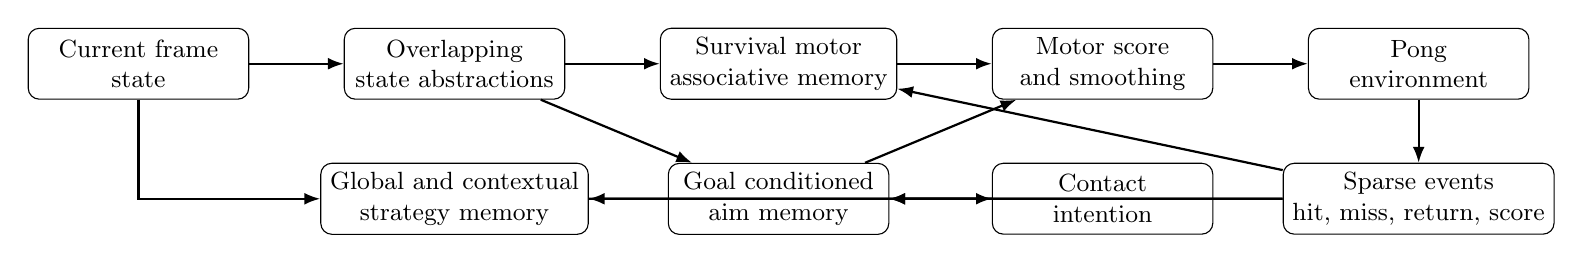
\begin{tikzpicture}[node distance=8mm and 12mm, every node/.style={font=\small}, box/.style={draw,rounded corners,align=center,minimum height=9mm,minimum width=28mm}, arr/.style={-{Latex[length=2mm]},thick}]
\node[box] (obs) {Current frame\\state};
\node[box,right=of obs] (keys) {Overlapping\\state abstractions};
\node[box,right=of keys] (surv) {Survival motor\\associative memory};
\node[box,below=of surv] (aim) {Goal conditioned\\aim memory};
\node[box,right=of surv] (motor) {Motor score\\and smoothing};
\node[box,right=of motor] (env) {Pong\\environment};
\node[box,below=of keys] (strat) {Global and contextual\\strategy memory};
\node[box,below=of motor] (intent) {Contact\\intention};
\node[box,below=of env] (events) {Sparse events\\hit, miss, return, score};
\draw[arr] (obs) -- (keys);
\draw[arr] (keys) -- (surv);
\draw[arr] (keys) -- (aim);
\draw[arr] (surv) -- (motor);
\draw[arr] (aim) -- (motor);
\draw[arr] (motor) -- (env);
\draw[arr] (env) -- (events);
\draw[arr] (events) -- (surv);
\draw[arr] (events) -- (aim);
\draw[arr] (events) -- (strat);
\draw[arr] (strat) -- (intent);
\draw[arr] (intent) -- (aim);
\draw[arr] (obs) |- (strat);
\end{tikzpicture}%
}
\caption{SEM architecture. Current observations address overlapping associative keys. Survival and aim memories jointly choose a motor action. Sparse physical outcomes update bounded eligibility traces. A separate opponent response memory selects contact intention. No module computes an analytical future ball intersection.}
\label{fig:architecture}
\end{figure*}

\section{Experimental Protocol}
\subsection{Training curriculum}
The main checkpoint was trained across 40 sequential runs of 55 incoming outcomes each, for 2,200 incoming outcomes total. The same SEM instance continued learning across runs; environment and coach seeds varied between runs. Runs used varied environment seeds and engineered coach opponents with center, spinner, top biased, bottom biased, mixed, and alternating styles. The first 35\% of runs used neutral contact intention to prioritize interception. The next 55\% used random intentions to train reusable contact control. The final 10\% used the learned strategy intention. Exploration remained active during training and decayed with accumulated motor outcomes.

After training, interception was evaluated with exploration disabled, fresh environment seeds, fresh strategy memories, and neutral contact intention. Contact control was evaluated separately using random intentions. Unless stated otherwise, benchmark comparisons use paired random seeds.

\subsection{Source audit and claim boundary}
An abstract syntax tree audit of the agent source searched for analytical future path solver signatures, future target variables, division by horizontal ball velocity, and neural framework imports. The validation report found none. This does not imply absence of inductive bias. SEM is given current state variables, hand selected bins, a finite action vocabulary, reward functions, smoothing, and the incoming direction gate. Engine physics and engineered training opponents are external to SEM.

\subsection{Controlled ablations}
Four primary ablations isolate major components. The trace ablation compares the full decaying motor eligibility trace with credit assigned only to the last decision. The aim ablation sets the aim residual weight to zero. The fast memory ablation removes fast strategy readout during a hidden opponent switch. The context ablation is evaluated on a deliberately conflicting benchmark in which the same contact direction has opposite value in two observable opponent contexts.

Further tests examine sensor ambiguity, shifted physics, overlapping abstraction transfer, hidden actuator reversal, and reacquisition savings. We report seed consistency and effect magnitudes rather than null hypothesis significance tests because the experiments are small, deterministic controlled benchmarks intended for mechanistic diagnosis.

\section{Results}
\subsection{Sparse outcome motor learning}
Figure~\ref{fig:training} shows the 40 run training trajectory. Hit rate rises from 0.709 in the first run to 0.964 by run 4 and reaches 1.0 in several subsequent runs. Across all training outcomes the lifetime hit rate is 0.958. Frozen evaluation on six fresh seeds yields a mean hit rate of 0.974. A separate validation suite on four fresh seeds measures an early miss count of 13.5 versus 3.75 late misses, a 72.2\% reduction.

\begin{figure}[t]
\centering
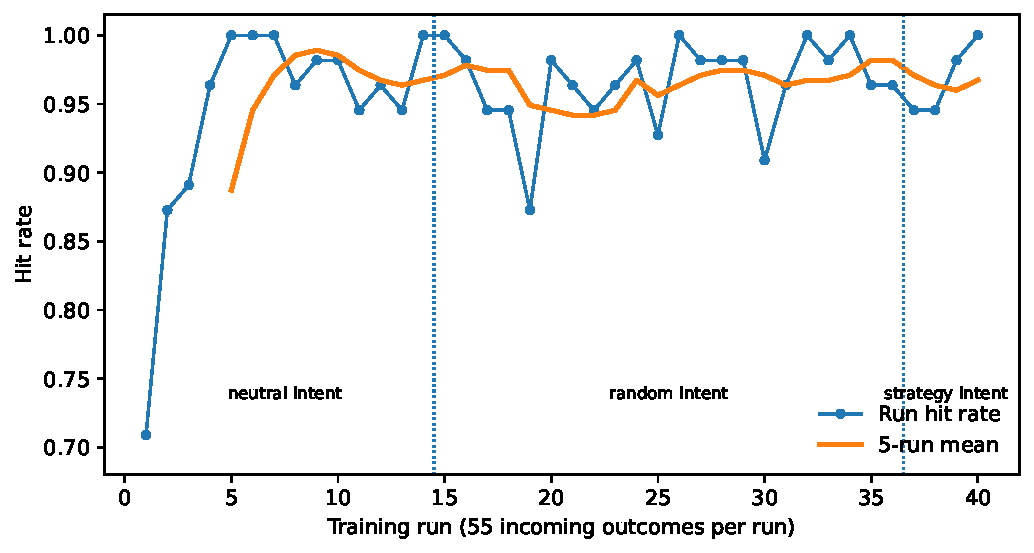
\includegraphics[width=\columnwidth]{figures/training_curve.pdf}
\caption{Motor performance over the 40 run curriculum. Each run contains 55 incoming outcomes. The orange line is a five run moving mean. Vertical lines mark changes in contact intention curriculum.}
\label{fig:training}
\end{figure}

The frozen controller on fresh evaluation seeds is not perfectly stable. The six seed evaluation records about 25.1 velocity sign changes per 1,000 incoming frames. This metric is used only as a rough smoothness diagnostic and is not optimized directly.

\subsection{Component ablations}
Table~\ref{tab:ablations} summarizes the strongest controlled ablations. Full eligibility traces reduce late misses relative to last decision credit in 7 of 8 seeds. The aim residual changes physical contact as intended: correlation between requested and actual contact is 0.395 with the aim memory and $-0.020$ without it, while interception remains high in both cases. This separates the survival objective from the contact execution objective.

Fast strategy values matter primarily after a contingency switch. In a hidden A to B opponent change, full memory reaches the predefined adaptation threshold in all six seeds with mean latency 23.2 outcomes. A slow only readout adapts in 4 of 6 seeds within the 100 outcome phase, with 63.3 outcome mean latency among successful runs. In the initial stationary phase, latency is nearly identical, which suggests the fast estimate contributes specifically to nonstationary adaptation rather than merely increasing stationary performance.

\begin{table}[t]
\centering
\caption{Primary controlled ablations. Values are means across paired seeds.}
\label{tab:ablations}
\small
\begin{tabular}{@{}p{0.31\columnwidth}p{0.29\columnwidth}p{0.29\columnwidth}@{}}
\toprule
Test & Full SEM & Ablated condition\\
\midrule
Motor trace, late hit & 0.869 & 0.697 last decision only\\
Aim, intent contact correlation & 0.395 & $-0.020$ no aim\\
Aim, contact MAE & 0.421 & 0.596 no aim\\
Hidden switch B latency & 23.2, 6/6 adapted & 63.3, 4/6 slow only\\
Context target intent, last 100 & 0.913 & 0.468 global only\\
Direction ambiguity, late hit & 0.963 & 0.594 no $v_y$\\
\bottomrule
\end{tabular}
\end{table}

\subsection{Hidden opponent change}
The opponent switch benchmark creates three 100 outcome phases: weak upward returns, weak downward returns, then weak upward returns again. SEM receives no phase label or switch signal, and strategy memory is reset only once before the first phase. Figure~\ref{fig:switch} shows the target contact preference. Across six seeds the first 20 to last 20 target fractions are 0.658 to 0.942 in A1, 0.458 to 0.875 in B, and 0.533 to 0.933 in A2. Mean adaptation latencies are 20.8, 23.2, and 23.5 outcomes respectively.

\begin{figure}[t]
\centering
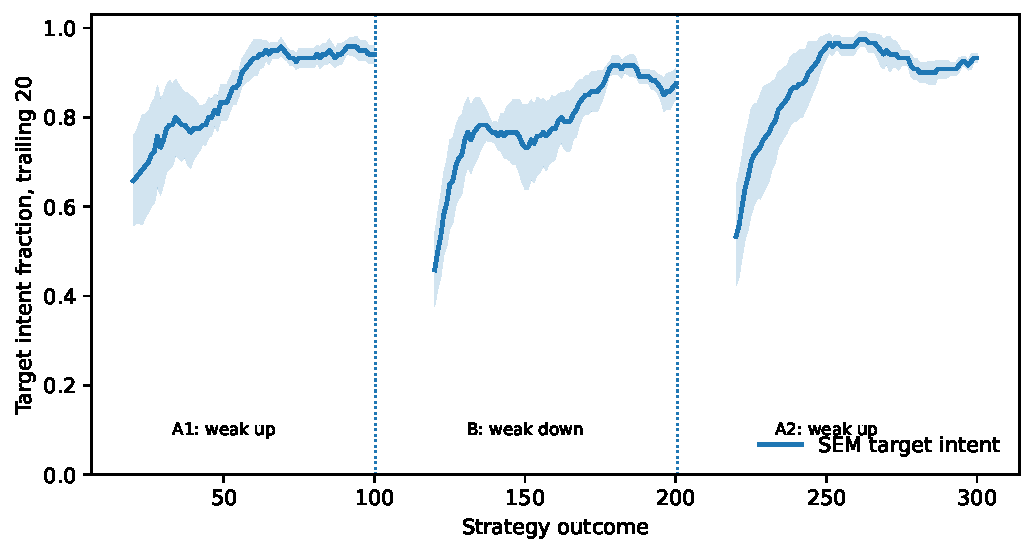
\includegraphics[width=\columnwidth]{figures/hidden_opponent_switch.pdf}
\caption{Online strategy adaptation after two hidden changes in opponent response statistics. Curves show mean trailing 20 target intention fraction across six seeds, with standard error bands. Rolling windows restart at phase boundaries.}
\label{fig:switch}
\end{figure}

The benchmark's reward landscape is external to SEM. Shots that actually enter the currently vulnerable trajectory family produce opponent misses about 42\% to 48\% of the time, compared with about 4\% to 7\% for other families. SEM therefore adapts to changed consequences rather than observing a benchmark mode label.

\subsection{Context dependent strategy}
A simpler hidden switch can be solved by global statistics alone, so it does not isolate contextual memory. We therefore constructed a conflicting contingency benchmark. Each trial exposes one of two balanced opponent paddle contexts. In one context positive contact is advantageous; in the other, negative contact is advantageous. The mapping is never given to SEM.

Over eight seeds and 320 trials per condition, full context memory selects the correct context dependent intention on 91.25\% of the last 100 trials. Global only memory reaches 46.75\%, near the expected conflict level. The full system is better in all 8 seeds. Figure~\ref{fig:context} shows learning over time.

\begin{figure}[t]
\centering
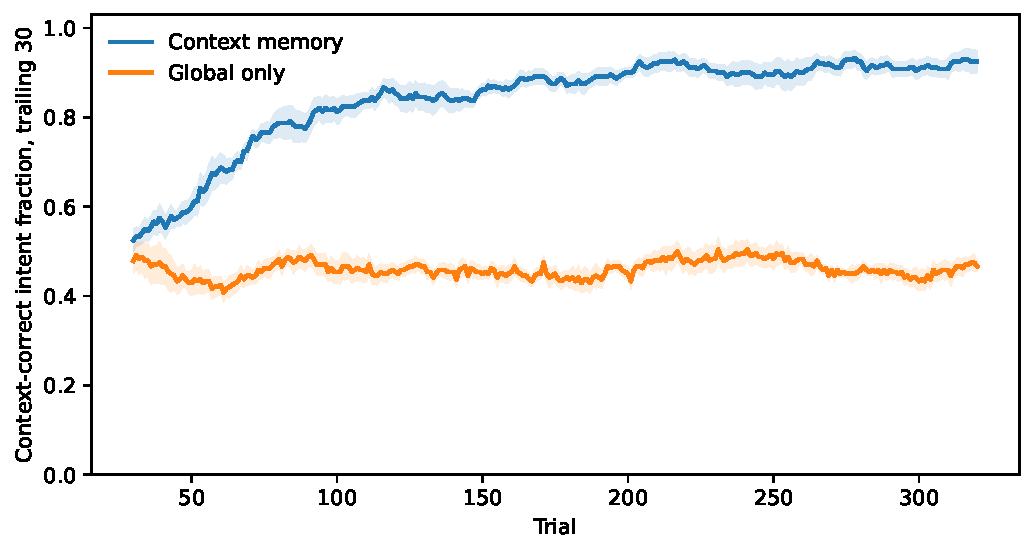
\includegraphics[width=\columnwidth]{figures/context_conditional_learning.pdf}
\caption{Context dependent conflicting contingency benchmark. The same action sign has opposite value in two observable contexts. Context specific memory learns the conditional mapping; global only memory cannot consistently resolve the conflict. Mean trailing 30 fraction across eight seeds with standard error bands.}
\label{fig:context}
\end{figure}

\subsection{The learned controller uses vertical velocity when geometry is ambiguous}
Removing vertical ball velocity from ordinary fresh Pong learning does not reduce performance. Late hit rate is 0.894 with the full state and 0.922 without vertical velocity, indicating that position, relative position, and distance often make the direction redundant and that additional bins can fragment data.

A controlled ambiguity benchmark removes this confound. Every trial begins with nearly identical ball and paddle geometry close to SEM, while $v_y$ is either $+700$ or $-700$. Sparse hit or miss reward remains unchanged. Across eight seeds, full state reaches 0.963 late hit rate and 0.953 first action direction accuracy. Removing vertical velocity yields 0.594 and 0.339 respectively, with full state superior in all eight seeds. Because no direct velocity-to-action rule is encoded in the controller, these results show that the learned action values can exploit $v_y$ when geometry alone is ambiguous.

\section{Generalization Through Overlapping Abstractions}
\label{sec:generalization}
The pretrained checkpoint was frozen and evaluated under physical changes that were never signaled to SEM. No action value was updated during these tests. Figure~\ref{fig:physics} shows six seed means. Hit rate remains 0.938 under a much faster ball, 0.960 under a slower actuator, and 0.921 under a hard compound shift that simultaneously changes field height, paddle height, maximum paddle speed, base and maximum ball speed, acceleration, and bounce angle scale.

\begin{figure}[t]
\centering
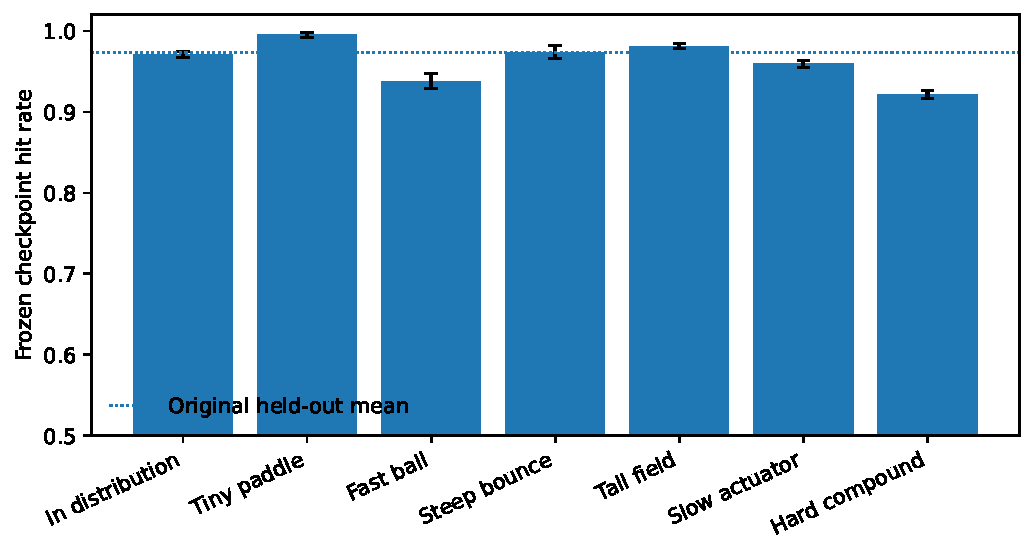
\includegraphics[width=\columnwidth]{figures/physics_generalization.pdf}
\caption{Frozen checkpoint under shifted physics. Bars show means across six paired seeds with standard error. The dotted line is the original six-seed fresh-evaluation mean from the training report.}
\label{fig:physics}
\end{figure}

The hard compound condition is particularly useful because the most specific state key was observed in training for only 57.2\% of decisions, while at least one coarser abstraction was available for all decisions. This suggests a route for transfer but does not by itself establish causality.

We therefore ablated the representation while keeping the checkpoint frozen and disabling the aim residual. With full overlapping keys, hit rate is 0.983 in distribution and 0.945 under hard compound physics. Using only the most specific key collapses performance to 0.681 and 0.564. Using only the coarser keys retains 0.979 and 0.929. On episodes containing unseen specific keys under hard compound physics, the corresponding rates are 0.944, 0.536, and 0.926.

\begin{figure}[t]
\centering
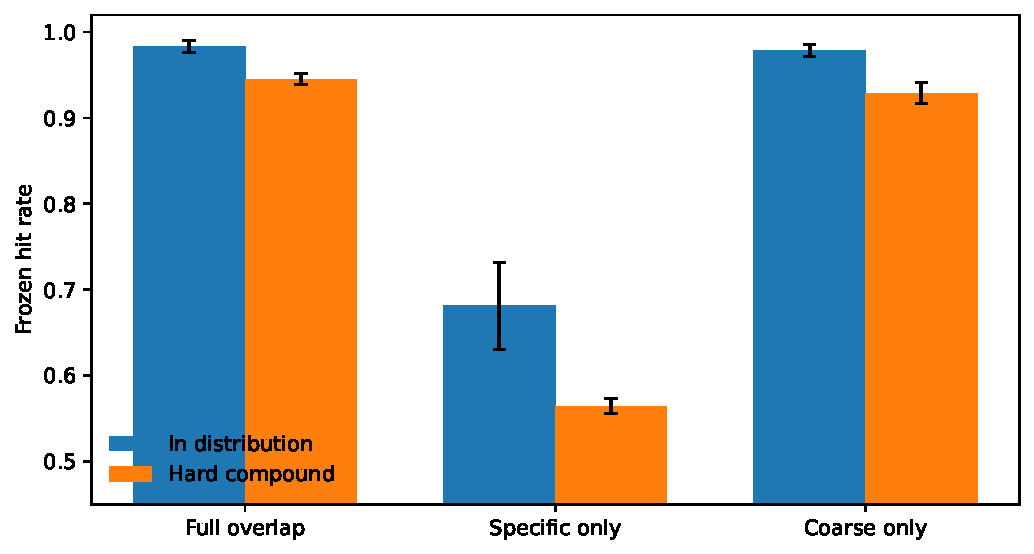
\includegraphics[width=\columnwidth]{figures/abstraction_transfer.pdf}
\caption{Frozen abstraction transfer ablation. Coarse overlapping keys preserve nearly all full performance, whereas a specific key only view degrades sharply, especially under shifted physics. Error bars are standard errors across six seeds.}
\label{fig:abstraction}
\end{figure}

These results are inconsistent with an explanation based solely on exact fine-grained state-action lookup. They do not imply representation learning: the abstractions themselves are hand designed.

\section{Continual Adaptation and Retention}
\label{sec:continual}
\subsection{Hidden actuator reversal}
To test adaptation at the motor consequence level, the environment secretly multiplies SEM's motor command by $-1$. The observation space is unchanged and SEM receives no remap indicator. A1 uses the normal actuator, B uses the inverted actuator for 220 outcomes, and A2 restores the normal actuator. Serve random number generation and coach behavior are paired across phases.

Figure~\ref{fig:remap} shows the resulting learning dynamics. Mean hit rate in the first 20 outcomes of B falls to 0.175 and rises to 0.733 in the final 20. When normal control returns, the corresponding recovery is 0.492 to 0.950. All six seeds improve from early to late in both B and A2.

\begin{figure}[t]
\centering
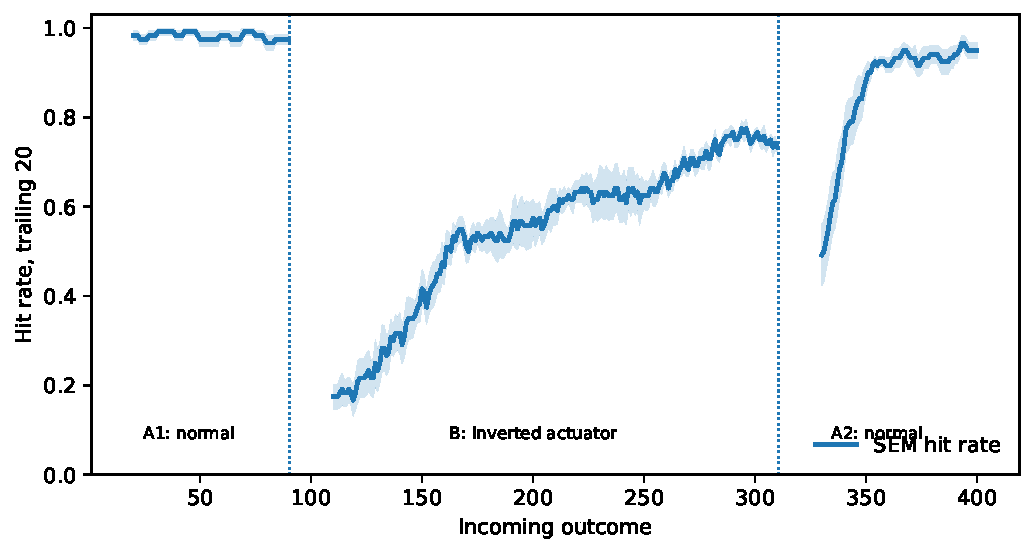
\includegraphics[width=\columnwidth]{figures/motor_remap_reversal.pdf}
\caption{Continual relearning after an unannounced reversal of the actuator mapping. Mean trailing 20 hit rate across six seeds with standard error bands. The agent receives no phase or mapping identifier.}
\label{fig:remap}
\end{figure}

The inverted mapping is not solved instantly, and final B performance remains below the original mapping. The result should therefore be interpreted as partial continual relearning, not instantaneous remapping.

\subsection{Reacquisition savings}
A second protocol uses A1 normal, B1 inverted, A2 normal, and B2 inverted, without resetting memory. B1 is the first inversion exposure and B2 is the repeated exposure. Across six seeds, mean latency to reach a 75\% rolling 20 hit criterion falls from 158.8 outcomes in B1 to 91.7 in B2. B2 reaches the threshold faster in all six seeds. First 50 hit rate rises from 0.243 to 0.407 and first 100 rate from 0.378 to 0.517.

A matched experience control receives the same quantity of pre target interaction but has never experienced inversion before its late B phase. The control reaches 0.230 in its first 50 and 0.365 in its first 100, below B2 in all six paired seeds. Among five runs in which both conditions cross the threshold, B2 is faster in four and tied in one; one additional control does not cross within the phase. Figure~\ref{fig:retention} compares the learning curves.

\begin{figure}[t]
\centering
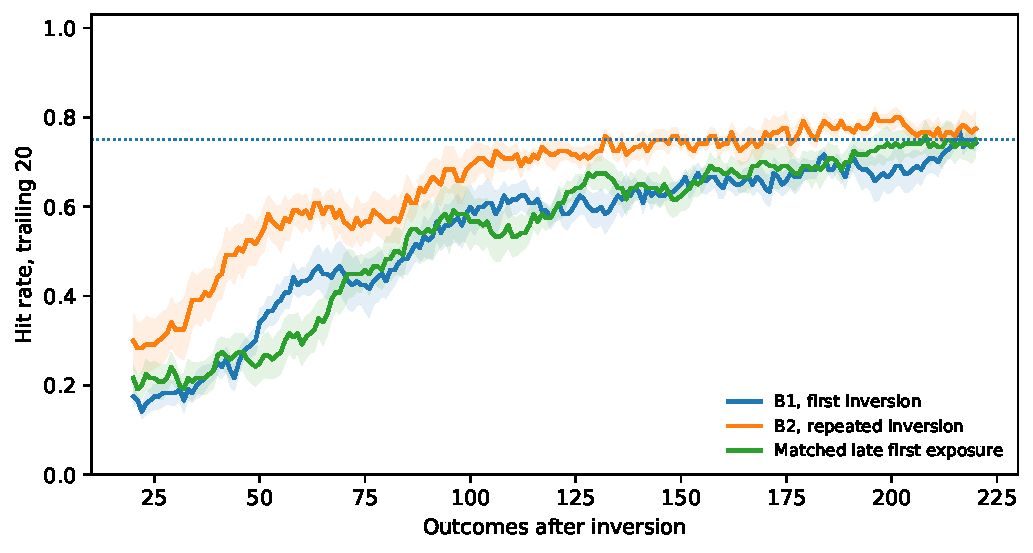
\includegraphics[width=\columnwidth]{figures/retention_savings.pdf}
\caption{Reacquisition savings after actuator inversion. Repeated inversion B2 improves faster than first inversion B1 and a matched experience agent encountering inversion for the first time. Mean trailing 20 hit rate across six seeds with standard error bands.}
\label{fig:retention}
\end{figure}

Savings weakens with interference. When only 40 normal mapping outcomes separate B1 and B2, B2 first 100 hit rate is 0.608 and threshold latency is 73.0. With 220 normal outcomes these become 0.465 and 104.2; with 440 they are 0.455 and 101.2. The 220 to 440 comparison does not show another large collapse, so a residual savings effect remains in these seeds.

A same history branch probe does not support the slow value estimate as the main retention carrier. After an identical A1, B1, A2 history, the agent is cloned at the B2 boundary. Full fast plus slow readout reaches 0.565 in the first 100, fast only reaches 0.622, and slow only reaches 0.382. Fast only adapts in all six seeds with mean threshold latency 67.7; slow only adapts in 2 of 6 seeds. The observed retention therefore appears more consistent with incompletely overwritten distributed action values across overlapping abstractions than with a dedicated slow store. This interpretation remains provisional because those internal values are not independently identified as memory traces.

\section{Discussion}
The central result is not that Pong can be solved without neural networks. Classical control, tabular reinforcement learning, coarse coding, and many engineered controllers already establish that neural networks are not required for simple control tasks. The more specific result is that a compact associative memory system can exhibit several behaviors that are often studied separately: sparse outcome motor learning, goal conditioned action modulation, context sensitive strategy, nonstationary adaptation, transfer through overlapping abstractions, hidden action consequence relearning, and measurable reacquisition savings.

The experiments also identify where simpler explanations are sufficient. Context memory provides little benefit when opponent weakness is globally consistent. It is required for high performance in the constructed conflicting-context benchmark, where the same action has opposite value in different observable contexts. Vertical velocity is similarly unnecessary in ordinary Pong but becomes necessary when current geometry is deliberately ambiguous. These negative controls are important because they prevent assigning mechanistic importance to a component simply because it is present in the architecture.

The slow value estimate is the weakest current element. It slightly reduces action preference switching under isolated noisy stationary rewards, but does not reliably improve long switch adaptation, temporary shock recovery, or motor retention. A stronger paper would be possible by removing it entirely or redesigning it, but this report retains the implemented architecture and states the evidence boundary explicitly.

SEM is also not equivalent to standard tabular Q learning. It does not maintain Bellman optimal action values or bootstrap from successor states. Its value entries are outcome associated exponential estimates written through a bounded eligibility trace. In that sense, the architecture is closer to an associative episodic control system with engineered coarse coding than to a conventional Markov decision process solver.

\section{Limitations}
The study is limited to a custom Pong environment and closely related controlled benchmarks. Generalization across physics parameters does not demonstrate transfer to a new task family. All observations are structured state variables rather than pixels. Binning, key construction, action sets, reward functions, exploration schedules, smoothing, and the incoming ball gate are hand engineered. Training opponents are also engineered curriculum generators.

The benchmark seed counts are small, usually between six and eight. The experiments are paired and often show complete seed consistency, but they are diagnostic rather than large scale statistical studies. No comparison is made with tuned tabular Q learning, tile coded Sarsa, model predictive control, DQN, or modern actor critic methods. Consequently, the work makes no claim of sample efficiency or performance superiority over established alternatives.

The source audit reduces the risk of an analytical trajectory solver being hidden in the agent, but it is not a formal proof of semantic absence of all oracle information. The environment itself of course implements Pong physics, and the current state includes velocity. Finally, the term structured episodic memory is descriptive of the architecture used here and should not be interpreted as a model of biological episodic memory.

\section{Conclusion}
The experiments show that, in the tested Pong setting, a carefully structured associative-memory controller can support useful online control and adaptation without a neural policy or a future trajectory solver. Within this setting, sparse temporal credit learns interception; a separate residual memory controls contact intention; context memory resolves conflicting action values; coarse overlapping abstractions support transfer when exact keys are unseen; and previously experienced actuator mappings are reacquired faster than matched first exposure.

The results are best viewed as an experimental systems study rather than a claim of a new reinforcement learning foundation. The strongest next step is not additional Pong tuning, but evaluation on a distinct control task with the same memory machinery and minimal task specific redesign. Such a transfer test would clarify whether SEM is a reusable architecture or a particularly effective decomposition for this environment.


\appendix
\section{Implementation Details}
\label{app:implementation}
This appendix records the principal implementation constants used in the released SEM v1.0 code. The purpose is reproducibility rather than introducing additional design claims. Unless an experiment explicitly ablates a component, these values are fixed across the reported benchmarks.

\subsection{Feature discretization and overlapping keys}
Let $d=(W-x_b)/W$ be normalized horizontal distance from the right boundary, $e=(y_b-y_p)/h_p$ be ball-to-paddle vertical offset in paddle-height units, $u=v_y/\max(v,1)$ be normalized vertical ball velocity, and $p_y=y_p/H$, $b_y=y_b/H$ be normalized paddle and ball heights. SEM discretizes these quantities with the thresholds in Table~\ref{tab:implbins}.

\begin{table*}[t]
\centering
\small
\caption{Fixed discretization thresholds used by the released implementation. Each feature index is the number of listed thresholds strictly below the current scalar value.}
\label{tab:implbins}
\begin{tabularx}{0.97\textwidth}{@{}l l X@{}}
\toprule
Feature & Symbol in code & Thresholds \\
\midrule
Fine distance & \texttt{xf} & $0.05, 0.10, 0.18, 0.28, 0.40, 0.55, 0.72, 0.90$ \\
Coarse distance & \texttt{xc} & $0.12, 0.30, 0.55, 0.80$ \\
Fine relative vertical offset & \texttt{ef} & $-1.80, -1.15, -0.72, -0.36, -0.12, 0.12, 0.36, 0.72, 1.15, 1.80$ \\
Coarse relative vertical offset & \texttt{ec} & $-1.05, -0.42, 0.42, 1.05$ \\
Fine normalized vertical velocity & \texttt{vf} & $-0.55, -0.18, 0.18, 0.55$ \\
Signed vertical velocity & \texttt{vs} & $-1$ for $u<-0.10$, $0$ for $|u|\leq0.10$, $+1$ for $u>0.10$ \\
Normalized paddle height & \texttt{py} & $0.18, 0.36, 0.55, 0.74, 0.90$ \\
Normalized ball height & \texttt{by} & $0.16, 0.34, 0.52, 0.70, 0.86$ \\
Ball speed & \texttt{sp} & $420, 560, 760, 940$ pixels s$^{-1}$ \\
\bottomrule
\end{tabularx}
\end{table*}

The survival motor table is addressed by five simultaneous keys, ordered from most specific to coarsest:
\begin{align*}
K_1 &= (\texttt{xf},\texttt{ef},\texttt{vf},\texttt{py},\texttt{by},\texttt{sp}),\\
K_2 &= (\texttt{xc},\texttt{ef},\texttt{vf},\texttt{py},\texttt{sp}),\\
K_3 &= (\texttt{xc},\texttt{ec},\texttt{vs},\texttt{sp}),\\
K_4 &= (\texttt{ef},\texttt{vf},\texttt{xc}),\\
K_5 &= (\texttt{ec},\texttt{vs}).
\end{align*}
Each tuple also carries a fixed type tag in code so that entries from different abstraction levels cannot collide. The aim table uses five analogous keys augmented by the nearest discrete contact intention and, for three of the keys, a discretized current geometric goal error $2e-g$. The fine goal-error thresholds are $-1.80,-1.15,-0.72,-0.38,-0.16,0.16,0.38,0.72,1.15,1.80$ and the coarse thresholds are $-0.90,-0.35,0.35,0.90$.

\subsection{Associative value readout}
For each key-action pair, SEM stores update count $n$, running arithmetic mean, fast estimate $F$, and slow estimate $S$. After the first observation initializes both estimates to target $z$, subsequent updates use
\begin{align}
F &\leftarrow 0.66F+0.34z,\\
S &\leftarrow 0.945S+0.055z.
\end{align}
For abstraction level $\ell\in\{0,1,2,3,4\}$, key-action readout weight is
\begin{equation}
w_{\ell}=\frac{1}{1+0.20\ell}\left[0.25+0.75\min\left(1,\frac{n}{7}\right)\right].
\end{equation}
The value contributed by that key is $0.70F+0.30S$. Evidence for an action is the sum of its counts over active keys. The survival table adds the exploration bonus
\begin{equation}
b(a)=0.17\sqrt{\frac{\log N}{1+E(a)}},
\end{equation}
where $E(a)$ is summed evidence and $N=\max(2,U+2)$ with $U$ the table's accumulated number of sparse trace updates. The aim residual uses the same weighted estimate but no uncertainty bonus.

Motor epsilon exploration is
\begin{equation}
\epsilon_m=\max\left(0.020,\;0.34\exp[-o/170]\right),
\end{equation}
where $o$ is the number of settled incoming motor outcomes; evaluation mode sets $\epsilon_m=0$. Ties among maximal scores are broken uniformly at random.

\subsection{Eligibility traces and actuator dynamics}
A trace step occurs once per motor decision, not once per rendered frame. Existing trace weights are multiplied by 0.88 in the survival trace and by 0.70 in the aim trace; entries below 0.045 are removed. Newly active key-action pairs are inserted with eligibility 1.0. The traces retain at most 84 and 48 items respectively. A hit writes survival target $+1.0$; a miss writes $-1.15$. The aim target on a hit is
\begin{equation}
r_{aim}=2\max\left(0,1-\frac{|c-g|}{1.05}\right)-1,
\end{equation}
and a miss writes $-0.70$. Each stored key-action pair receives the corresponding sparse target multiplied by its current eligibility.

Motor decisions are held for five rendered frames. For action $a$, the score used for greedy choice is
\begin{equation}
Q(a)=Q_{survival}(a)+1.05Q_{aim}(a)-0.055|a-a_{prev}|.
\end{equation}
The chosen discrete action is multiplied by the environment-provided maximum SEM paddle speed. Applied velocity is first-order smoothed as
\begin{equation}
v^{applied}_{t+1}=v^{applied}_{t}+0.28\left(v^{desired}_{t}-v^{applied}_{t}\right).
\end{equation}
Values with absolute magnitude below 1 pixel s$^{-1}$ are set to zero. The engineered incoming gate permits motor decisions only when $v_x>0$.

\subsection{Opponent-response strategy memory}
Strategy context is the tuple of opponent vertical-position bin, current ball-speed bin, and opponent-motion bin. Opponent position uses normalized thresholds $0.25,0.45,0.60,0.78$. Opponent velocity is estimated at 60 Hz and smoothed as $\hat v^{opp}_t=0.86\hat v^{opp}_{t-1}+0.14v^{measured}_t$; motion bins use thresholds $-120,-35,35,120$ pixels s$^{-1}$.

For contact action $a$, let $(F_g,S_g,n_g)$ denote global statistics and $(F_c,S_c,n_c)$ context statistics. Context weight is
\begin{equation}
\alpha_c=\min(0.72,n_c/7),
\end{equation}
and the deterministic strategy value before exploration bonus is
\begin{equation}
V(a)=(1-\alpha_c)(0.62F_g+0.38S_g)+\alpha_c(0.72F_c+0.28S_c).
\end{equation}
The strategy adds
\begin{equation}
0.15\sqrt{\frac{\log(N_g+1)}{n_g+1}},
\end{equation}
where $N_g=1+\sum_a n_g(a)$. Strategy epsilon is
\begin{equation}
\epsilon_s=\max\left(0.080,\;0.42\exp[-m/48]\right),
\end{equation}
with $m$ the number of settled SEM shots. If the opponent misses, strategy reward is $1.0$. If the opponent returns, the observed response is $\rho=\min(1,|c_{opp}|)$ and reward is $0.12+0.30\rho$. A point scored by the opponent while a SEM shot is pending gives strategy reward $0$.

\subsection{Reproducibility boundary}
The released checkpoint stores the survival and aim associative tables, motor outcome counters, and optionally strategy memory. Fresh-human play loads the pretrained motor checkpoint while resetting opponent strategy by default. Frozen evaluations disable epsilon exploration and prevent learning updates where specified by the benchmark script. Experiment scripts, random seeds, raw JSON outputs, and the exact checkpoint used for the figures are included in the release archive. The appendix describes the released implementation rather than a claimed optimal configuration; several experiments in the paper intentionally ablate these values or memory components.

\section*{Code and Data Availability}
\addcontentsline{toc}{section}{Code and Data Availability}
The source code, fixed experiment scripts, raw JSON outputs, figures, and a versioned archive are intended to accompany the public release of this report. Replace the placeholder below with the final project or Zenodo record after publication.

\begin{center}
\url{https://PLACEHOLDER-SEM-PROJECT-LINK}
\end{center}

\addcontentsline{toc}{section}{References}
\begin{thebibliography}{99}

\bibitem[Albus(1975)]{albus1975cmac}
J. S. Albus.
\newblock A new approach to manipulator control: The cerebellar model articulation controller (CMAC).
\newblock \emph{Journal of Dynamic Systems, Measurement, and Control}, 1975.
\newblock doi:10.1115/1.3426922.

\bibitem[Blundell et~al.(2016)Blundell, Uria, Pritzel, Li, Ruderman, Leibo, Rae, Wierstra, and Hassabis]{blundell2016mfec}
C. Blundell, B. Uria, A. Pritzel, Y. Li, A. Ruderman, J. Z. Leibo, J. Rae, D. Wierstra, and D. Hassabis.
\newblock Model-Free Episodic Control.
\newblock \emph{arXiv:1606.04460}, 2016.

\bibitem[Kirkpatrick et~al.(2017)Kirkpatrick, Pascanu, Rabinowitz, Veness, Desjardins, Rusu, Milan, Quan, Ramalho, Grabska-Barwinska, Hassabis, Clopath, Kumaran, and Hadsell]{kirkpatrick2017ewc}
J. Kirkpatrick et al.
\newblock Overcoming catastrophic forgetting in neural networks.
\newblock \emph{Proceedings of the National Academy of Sciences}, 114(13):3521--3526, 2017.
\newblock doi:10.1073/pnas.1611835114.

\bibitem[McCloskey and Cohen(1989)]{mccloskey1989catastrophic}
M. McCloskey and N. J. Cohen.
\newblock Catastrophic interference in connectionist networks: The sequential learning problem.
\newblock In \emph{Psychology of Learning and Motivation}, volume 24, pages 109--165. Academic Press, 1989.
\newblock doi:10.1016/S0079-7421(08)60536-8.

\bibitem[Mnih et~al.(2015)]{mnih2015dqn}
V. Mnih et al.
\newblock Human-level control through deep reinforcement learning.
\newblock \emph{Nature}, 518:529--533, 2015.
\newblock doi:10.1038/nature14236.


\bibitem[Moore and Atkeson(1992)]{moore1992memory}
A. W. Moore and C. G. Atkeson.
\newblock Memory-based reinforcement learning: Efficient computation with prioritized sweeping.
\newblock In \emph{Advances in Neural Information Processing Systems 5}, pages 263--270, 1992.

\bibitem[Moore and Atkeson(1993)]{moore1993prioritized}
A. W. Moore and C. G. Atkeson.
\newblock Prioritized sweeping: Reinforcement learning with less data and less real time.
\newblock \emph{Machine Learning}, 13:103--130, 1993.
\newblock doi:10.1007/BF00993104.

\bibitem[Ormoneit and Sen(2002)]{ormoneit2002kernel}
D. Ormoneit and S. Sen.
\newblock Kernel-based reinforcement learning.
\newblock \emph{Machine Learning}, 49(2--3):161--178, 2002.
\newblock doi:10.1023/A:1017928328829.

\bibitem[Pritzel et~al.(2017)Pritzel, Uria, Srinivasan, Puigdomenech Badia, Vinyals, Hassabis, Wierstra, and Blundell]{pritzel2017nec}
A. Pritzel, B. Uria, S. Srinivasan, A. Puigdomenech Badia, O. Vinyals, D. Hassabis, D. Wierstra, and C. Blundell.
\newblock Neural Episodic Control.
\newblock In \emph{Proceedings of the 34th International Conference on Machine Learning}, volume 70 of PMLR, pages 2827--2836, 2017.

\bibitem[Sutton(1988)]{sutton1988td}
R. S. Sutton.
\newblock Learning to predict by the methods of temporal differences.
\newblock \emph{Machine Learning}, 3:9--44, 1988.
\newblock doi:10.1007/BF00115009.

\bibitem[Sutton(1996)]{sutton1996coarse}
R. S. Sutton.
\newblock Generalization in reinforcement learning: Successful examples using sparse coarse coding.
\newblock In \emph{Advances in Neural Information Processing Systems 8}, pages 1038--1044. MIT Press, 1996.

\bibitem[Sutton and Barto(2018)]{sutton2018rl}
R. S. Sutton and A. G. Barto.
\newblock \emph{Reinforcement Learning: An Introduction}.
\newblock MIT Press, second edition, 2018.


\bibitem[Unemi(1992)]{unemi1992instance}
T. Unemi.
\newblock Instance-based reinforcement learning method.
\newblock \emph{Journal of the Japanese Society for Artificial Intelligence}, 7(4):697--707, 1992.
\newblock doi:10.11517/jjsai.7.4\_697.

\bibitem[Watkins and Dayan(1992)]{watkins1992q}
C. J. C. H. Watkins and P. Dayan.
\newblock Q-learning.
\newblock \emph{Machine Learning}, 8:279--292, 1992.
\newblock doi:10.1007/BF00992698.

\end{thebibliography}

\end{document}
